
% Many thanks to Andrew West for writing most of this file
% Main LaTeX file for CIS400/401 Project Proposal Specification
%
% Once built and in PDF form this document outlines the format of a
% project proposal. However, in raw (.tex) form, we also try to
% comment on some basic LaTeX technique. This is not intended to be a
% LaTeX tutorial, instead just (1) a use-case thereof, and (2) a
% template for your own writing.

% Ordinarily we'd begin by specifying some broad document properties
% like font-size, page-size, margins, etc. -- We have done this (and
% much more) for you by creating a 'style file', which the
% 'documentclass' command references.
\documentclass{sig-alternate}
 
% These 'usepackage' commands are a way of importing additional LaTeX
% styles and formattings that aren't part of the 'standard library'
\usepackage{mdwlist}
\usepackage{url}

\begin{document} 

% We setup the parameters to our title header before 'making' it. Note
% that your proposals should have actual titles, not the generic one
% we have here.
\title{CIS400/401 ARMS: Augmented Reality for Math and Science}
\subtitle{Dept. of CIS - Senior Design 2013-2014\thanks{Advisor: Boon Loo (boonloo@cis.upenn.edu).}}
\numberofauthors{4}

\author{
Allison Pearce \\ \email{alpearce@seas.upenn.edu} \\ Univ. of Pennsylvania \\ Philadelphia, PA
\and Spencer Lee \\ \email{lesp@seas.upenn.edu} \\ Univ. of Pennsylvania \\ Philadelphia, PA
\and Tanvir Ahmed \\ \email{tanvir@seas.upenn.edu} \\ Univ. of Pennsylvania \\ Philadelphia, PA
\and Will McDermid \\ \email{wmcd@seas.upenn.edu} \\ Univ. of Pennsylvania \\ Philadelphia, PA}

\date{}
\maketitle

% Next we write out our abstract -- generally a two paragraph maximum,
% executive summary of the motivation and contributions of the work.
\begin{abstract}
  \textit{We propose a mobile augmented reality application to help demonstrate math and physics concepts to middle and high school students.  Our primary motivation for this project is to make math and physics principles more tangible and more interesting to students using technology that many of them already own. Similar applications have been demonstrated to be effective for learning, but most previous work has relied on custom hardware. We aim to bring this technology to a mobile platform, making it more accessible to students and advancing the state of the art in mobile augmented reality applications for education.}

\end{abstract}

% Then we proceed into the body of the report itself. The effect of
% the 'section' command is obvious, but also notice 'label'. Its good
% practice to label every (sub)-section, graph, equation etc. -- this
% gives us a way to dynamically reference it later in the text via the
% 'ref' command.
\section{Introduction}
\label{sec:intro}
Augmented reality (AR) is a technology that allows users to perceive and interact with completely computational objects in the real world. Previous literature defines three specific characteristics of an augmented reality system \cite{azuma2001recent}: 
\begin{enumerate}
\item It combines real and virtual objects in a real environment
\item It aligns real and virtual objects with each other
\item It is interactive, and runs in real time and three dimensions
\end{enumerate}
The definition of AR includes systems that interact with all five human senses, but the most common implementation uses a visual display, and these are the systems we will focus on. The simplest way to create visual AR is through a digital device with a camera that serves as a lens to the real world. While the user looks through the lens, an application overlays virtual objects on the video feed of the real environment. This is known as video see-through \cite{van2010survey}.  Other options are creating an AR overlay using mirrors and lenses, or projecting AR overlays onto real objects. Video see-through offers a number of advantages, including lowest cost and easiest implementation.  

Video see-through AR has recently become feasible on a widespread consumer scale, thanks to the popularity and rapid development of mobile platforms such as iOS and Android. This has opened up a profusion  of possible consumer applications of AR, including education.  Studies have demonstrated the benefits of AR in the classroom,  including engaging and motivating students, enabling hands-on learning where it would otherwise be impossible (i.e. astronomy), and providing a system students can use for independent learning at their own pace \cite{whatevs}. With math and physics in particular, augmented reality offers the advantage of allowing students to repeat experiments quickly and easily without the need for additional equipment. Furthermore, the three-dimensional aspect of AR allows for a more realistic representation of math and physics concepts -- such as volume, surface integrals, and three-dimensional motion -- than two-dimensional textbooks, graphing calculators, or online tutorials can offer.  Few such applications exist, and even fewer are available on mobile platforms. Many existing math and physics applications require special hardware such as a headpiece or stylus, and accessing the equipment often requires a visit to a lab \cite{kaufmann2003mathematics, kaufmann2008simulating}.  

We propose an application that will bring the benefits of AR for math, physics, and related subjects to cell phones and tablets, which many students, parents, and teachers already own. The app will serve as a supplement to classroom learning and will allow the student to interact with his or her notes, adding 3D animations, models, and diagrams to enhance their understanding of the material. We expect to make math and science concepts more understandable and more fun to learn by using a novel technology that requires no special hardware. This could have far-reaching impacts for secondary education. We also intend to overcome some of the existing challenges in developing augmented reality applications for mobile platforms, which will further the state of the art of mobile-based AR. 


% The header of this document might have been a little intimidatating
% to beginners. Notice once you are in the body of the document,
% however, LaTeX commands are minimal and 'normal text' is frequent.
\section{Related Work}
\label{sec:related_work}
Several projects already exist with the goal of utilizing augmented reality or virtual reality technology for educational purposes, however, these projects are either fully virtualized or require the use of expensive, custom-designed tracking and haptic hardware. Many of these projects were proposed and implemented in order to explore the potential of virtual reality or mixed reality for augmenting the learning process, as discussed by Mantovani in \cite{mantovani200112}. As evidenced by the evaluations of these projects, virtual or mixed reality demonstrations of concepts do seemingly enhance the learning experience, especially when these demonstrations are dynamic and interactive, and when the environment is immersive. Unfortunately, in order to achieve optimal immersiveness and interactivity, expensive hardware is required, which limits the accessibility of such technology. We will discuss in further detail some major related works which apply virtual or mixed reality approaches to math and science education, pointing out how these projects demonstrated the effectiveness of augmented learning, and also how these projects are not easily disseminated to a wide user base.

\subsection{Studierstube}
Studierstube \cite{schmalstieg2002studierstube} is an augmented reality framework upon which several other AR projects (such as PhysicsPlayground and Construct3D) are built. Studierstube focuses on collaborative AR, where separate users can interact with shared virtual entities that are embedded into a real-world environment. The developers of Studierstube believe that AR applications are more feasible for manipulating three-dimensional information in an educational environment than purely virtual applications. Studierstube is designed for use with head-mounted displays or projection screens, and the environment is controlled using a Personal Interaction Panel (PIP).

\subsection{CyberMath}
CyberMath \cite{taxen2001cybermath} is a shared virtual environment in which users can control personal avatars and explore an area similar to museum in which mathematical concepts are visually demonstrated. Cybermath is built on the DIVE framework \cite{carlsson1993dive}. Users can interact with the different exhibits in order to explore and attain a greater understanding of the demonstrated concepts. Additionally, there is a central hub which can be used for more traditional teaching methods, such as lecturing and presenting slideshows. CyberMath contained four completed exhibitions in 2001:
\begin{itemize}
\item Interactive transformations, where users can map a three-dimensional domain point to a range point and investigate the effects of these mappings on different entities such as points, lines, planes, spheres, and rectangular prisms.
\item Generalized cylinders, where users can construct three-dimensional surfaces using differential geometry. Differential geometry is usually an advanced topic, but aspects can be demonstrated with relative ease.
\item Cylindrical optics, where cylindrical mirrors can be positioned and bent in order to demonstrate the reflection and focusing of waveforms.
\item Focal surfaces, in which focal sheets (another differential geometry concept) are shown for a given surface.
\end{itemize}
CyberMath, being a purely virtual environment,  lacks the immersiveness and tangibility of an AR application.

\subsection{PhysicsPlayground}
PhysicsPlayground \cite{kaufmann2008simulating} is an AR application in which students and teachers can create physical experiments that can be simulated in real time in a virtual environment. PhysicsPlayground is built on top of the Studierstube AR framework and uses the PhysX API as its physics engine. Students are able to walk around objects and view experiments from different perspectives, providing a highly immersive experience. Being able to simulate experiments in real time encourages students and teachers reconfigure and variate experiment parameters. Because PhysicsPlayground is based on Studierstube, it also requires the use of HMDs and a PIP to interact with the virtual environment. Both PhysicsPlayground and Construct3D were developed in the same lab.

\subsection{Construct3D}
Construct3D \cite{kaufmann2003mathematics} is an AR application built on the Studierstube framework, which focuses on extending the realm of differential geometry in order to improve spatial skills of students in high school or other higher education. Construct3D was evaluated over 500 users, which included students, teachers, and experts, over the course of five years \cite{tuw176085}. Construct3D allows users to dynamically construct and interact with three-dimensional entities in three-dimensional space. Users are able to construct primitives such as points, lines, planes, cubes, spheres, cylinders, cones, b-splines, b-spline surfaces, conic sections, and quadratics, among others. Operations on these primitives include but are not limited to boolean operations (intersection, difference, union, etc.), normal lines/planes, symmetry operations, and measurements. Objects are constructed in 3D layers, where overlapping subspaces can be controlled and viewed separately by each user. 

Different hardware environments were evaluated for use with Construct3D, in addition to the wearable setup with HMD and PIP, projection screens setups and personal workstations were also used. These alternative setups lack the same level of immersion that HMDs provide. The HMDs used with Construct3D are described in more detail in \cite{kaufmann2007multiple}, and their drawbacks are discussed in the evaluation of Construct3D \cite{kaufmann2007summary}. Primarily, head-mounted displays have a propensity for causing ``simulator sickness" when used for extended durations. Some students reported experiencing eye strain and headache after 20 minutes. 

Other major obstacles preventing technology such as Construct3D from becoming widely used in education environments are brought to attention by H. Kaufmann in \cite{tuw176085}:
\begin{itemize}
\item The costs of the hardware and software environment are too high
\item There is need for specialized maintenance of all equipment, which further increases costs
\item The most efficient and preferred setup supports only 2-3 users simultaneously
\end{itemize}
We hope to address these three obstacles directly with our project.

\section{Project Proposal}
\label{sec:project_proposal}
Our project aims to help students understand concepts in mathematics and science better through the aid of an augmented reality application running on easily accessible hardware. To this end, our application will provide visuals in terms of graphs, 3D images, definitions, and demonstrations alongside text such as a student's notes that will improve comprehension of the material at hand. What is unique about our project is that we will target our application to run on iOS devices because they are now ubiquitous and will not require most of our user-base to acquire additional sophisticated hardware.

Although educational support with AR has been attempted by others in the field, their efforts had little impact because they required the purchase of additional hardware or extra materials. For example, most AR applications in the education field today use special cards or markings that tell the AR application that this is an area of interest, or even relied on a unique headpiece. Our application will use equations or keywords in text to signal when to begin processing information, and to determine what to display. This is will allow us to create a general-purpose application that is not confined to a few use cases. It also means that there is no additional overhead into making a block of text �AR compatible�.  We hope that this will help students better understand the material that they are working on by providing in-line aid without extra effort from the publisher or student. 

A particular use case in mathematics could be a student struggling with 3D graphs. Using our application, he could launch our application on his iPhone and point the camera at an equation in his notes. Our applicatoin would overlay a graph of the surface described by the equation on his notepaper. Similarly, imagine a demonstration of projectile motion on the table next to a student's physics notes. Or even in computer science, imagine a student is reading about merge sort for the first time. For some, this may be a difficult algorithm to visualize. Our app will pull up and overlay an animation depicting merge sort onto the user�s paper. These aids will make it easier and more fun for middle and high school students to learn math and science.   

%A particular use case in the field of Computer Science would be when a student is reading about merge sort for the first time. For some, this may be a difficult algorithm to visualize. With our application, a user would launch the iOS application and point the device�s camera at text describing merge sort. Our app will then pull up and overlay a graphic or animation depicting merge sort onto the user�s paper. This would require no additional work from the user�s end in terms of marking the text, etc.


\subsection{Anticipated Approach}
\label{subsec:approach}

We will develop an iOS application to serve as a light client and input device. Users will launch the app and point the device�s camera at the text s/he would like to visualize. The device�s camera will then analyze the images at a fixed rate, attempting to perform OCR on the text. Once the OCR algorithm is successful, the data will be sent to the cloud for further processing. This will be done by attaching the information as a JSON object to the body of a POST request.

In the cloud, the text input will be analyzed to determine possible graphics for display. This will be done by reducing the text into possible points of interest (a math formula, important keywords) and comparing them against a repository of stored results for queries. If there is a match, then we will send the image�s url (stored on our servers) to the device. Otherwise, if the type of the text is a math formula, then we will feed it through a formula visualizer and generate an image which we will associate with the formula and stored on our servers. The url for the new image will then be sent to the device.

Back on the device, the image will be downloaded and cached while the iOS application determines the best location at which to overlay the image over the user�s paper. This will be done through image processing to find an area with a maximum of negative space. Once the optimal location is found, the image will be overlaid at the location. If the image would overlap text then the opacity of the image will be reduced so as to leave the text legible.

\begin{figure}[htb!]
	\begin{center}
		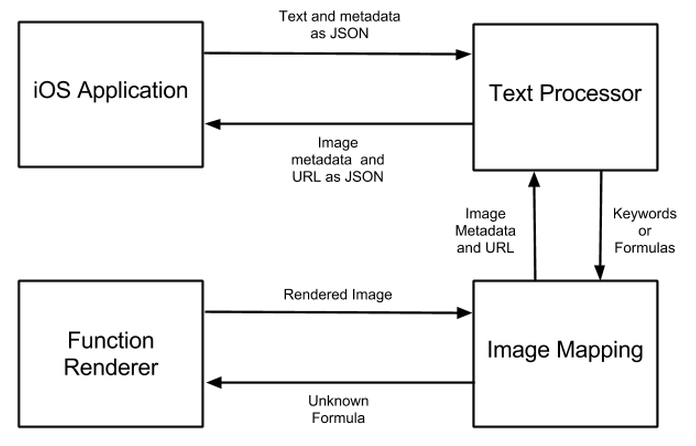
\includegraphics[width=0.9\linewidth]{block_diagram}
	\end{center}
	\vspace{-12pt}
	\caption{Example Figure/Graph}
	\label{fig:some_graph}
\end{figure}
\subsection{Technical Challenges}
\label{subsec:tech_challenges}

Implementing a reliable system of this scope will present several interesting challenges. We will need to perform OCR on an image the user chooses without any user input. This will need to be done both quickly and reliably, and on the device to prevent the network latency inherent in sending a cluster of images over the network. 

Once on our servers, the text will need to be parsed for points of interest. Apart from actually determining the points of interest, we will need to implement some similarity metrics if we are going to use them (the points of interest) to index into an image mapping. To continue with our merge sort use case, ``merge sort" and ``mergesort" should index to the same image.

Another challenge will be finding appropriate images for non-formula inputs, or for formula inputs which cannot be visualized in two or three dimensions. When the image cannot be rendered with our Formula Renderer module, we will need to display something to the user. This can perhaps be done through manual loading of images or through some image search over the web.

Finally, there is the issue of displaying the image to the resulting image to the user. This must be done in an unobtrusive and helpful way, and will likely involve image processing and optimization for negative space. In cases where there is very little negative space, the opacity of the image must be adjusted to allow the original image to be seen even after the application's image is displayed. Determining the optimal settings for position and opacity will be difficult.

\subsection{Evaluation Criteria}
\label{subsec:eval_criteria}
Since our project aims to help students understand concepts in mathematics and science, we would evaluate our project to see how well we could help students understand these concepts as well as evaluate against current AR standards. 

For the actual AR application, we want to be able to create a system that works seamlessly. To that end, we want to be able to reduce the latency between aiming the lens at an area of interest and the corresponding material being displayed in the application. This means that we will have to minimize the delay between detecting an area of interest in the real world, processing the area of interest and uploading its contents to our servers, determining what visual aid will help in this situation, responding to the client, and displaying the content to the user. Currently, system delay is a huge barrier for AR in the education space.  According to Handbook of Research on Educational Communications and Technology, system delay makes the virtual images ``lag behind" the real world which make them seem to ``swim around" \cite{jonassen2013handbook}. This has adverse effects on education as it inhibits registration, which is the ability for the human mind to recognize and track a particular object. We want to hit a target of a 4 second delay for our system from end to end. This is our goal since the processing for the data needs to be done in the cloud.

We also need to evaluate ourselves on our performance on our platforms of choice. Specifically, we would test to make sure that our app runs smoothly on iOS devices. We hope to run our application using less than 80\% of the CPU on these devices. To test this, we can use Instruments in the Xcode IDE to check how much CPU our application is using. We target 80\% because this would make sure that our app does not use too many resources and that it would prolong battery life.

To test usability and effectiveness, we would visit a school in Philadelphia and allow students there to use our application. We will conduct a survey amongst the students to see whether our application helped their ability to understand concepts in math and science. Our goal from this experiment would be to achieve an overall 40\% improvement. That is, have at least 4 out of every 10 children claim that it was easier to understand the concepts at hand. 

We would first pick out two concepts that are typically difficult to understand given text and normal diagrams. For the first trial, we will pick two concepts that are explained using sentences or paragraphs of text without any diagrams. We will give each student the first concept and check to see how well they understand the material. We will then give them the second concept and our application to see how well they understand the material with the new visual aid. Then, we can repeat the experiment with two new concepts, but with diagrams this time. We would test whether or not our application can generate unique aids as well as whether our app is helpful in situations where there are already diagrams present. 

Another thing that we can do is test the actual user interface of our final product. Since we want to make it easier for students to understand material, we need to make our application so that it is easy to use. We will conduct simple usability experiments to test whether or not users are able to find everything useful within our app and conduct a survey to check whether or not the app was easy to use.

\section{Research Timeline}
\label{sec:research_timeline}
Finally, we would like you to speculate about the pace of your
research progress. This section need not be lengthy, we would just
like you to specify some milestones so we can gauge your progress
during our intermediate interviews. Let us follow through with our
image recognition example:

% The 'itemize' environment shown here, and its friend 'enumerate'
% (shown below), are used to create indented\bulleted\outline style
% lists.

Already done
Performed research on augmented reality. Began looking into OCR libraries, function renderers, and Natural Language Processing libraries.
By Thanksgiving break
Have a basic function renderer working in the cloud.
By Christmas break
Have basic OCR working and sending information to servers. iOS application can display images (without choosing optimal location/opacity)
By the start of Spring term
Have simple NLP working. Finished OCR and function renderer.
By the end of March
Have NLP working and choosing points of interest. Have basic image search working. iOS application can position images based on negative space.
Reach goals
Choose optimal opacity for rendered images based on amount of negative space. Allow users to interact with rendered images (rotate views of 3D functions, for example).


\begin{itemize*}
	\item {\sc already completed}: Performed research on augmented reality. Began looking into OCR libraries, function renderers, and Natural Language Processing libraries.\vspace{3pt}
	\item {\sc prior to thanksgiving} : Have a basic function renderer working in the cloud.\vspace{3pt}
	\item {\sc prior to christmas} : Have basic OCR working and sending information to servers. iOS application can display images (without choosing optimal location/opacity).\vspace{3pt}
\item {\sc by the start of spring term} : Have simple NLP working. Finished OCR and function renderer.\vspace{3pt}	
\item {\sc by the end of march} : Have NLP working and choosing points of interest. Have basic image search working. iOS application can position images based on negative space.\vspace{3pt}
\item {\sc reach goals} : Choose optimal opacity for rendered images based on amount of negative space. Allow users to interact with rendered images (rotate views of 3D functions, for example). \vspace{3pt}
\item {\sc completion tasks} : Verify implementation is meets requirements. Conduct effectiveness and ease of use testing. Complete write-up.\vspace{3pt}
\item {\sc if there's time} : Investigate machine learning techniques to display more useful content.
\end{itemize*}

% We next move onto the bibliography.
\bibliographystyle{plain} % Please do not change the bib-style
\bibliography{prop_spec}  % Just the *.BIB filename

% Here is a dirty hack. We insert so much vertical space that the
% appendices, which want to begin in the left colunm underneath
% "references", are pushed over to the right-hand column. If we looked
% hard enough, there is probably a command to do exactly this (and
% wouldn't need tweaked after edits).
\vspace{175pt}

% We then use appendices to share some additional information with
% you, though you won't need appendices in your own proposal.

% The usage of 'enumerate' (similar to 'itemize') we talked about
% above

% You may also notice we have many 'vspace' commands lying
% around. These create 'vertical space' and are a way to force LaTeX
% to cooperate, sometimes. Don't get too involved with using them
% initially, though, because adding or deleting a single line of task
% can dramatically change how LaTeX chooses to format, page, and space
% the document
\end{document} 

